% !TeX spellcheck = en_US

\chapter{Trees}

\section {General Trees}

A \textbf{tree} is an abstract data type that organize  elements hierarchically.

A tree is \textbf{ordered} if there is a meaningful order among the children of each node.

\section{Binary Tree}

A \textbf{binary tree} is an ordered tree in which any node could have at most 2 children.

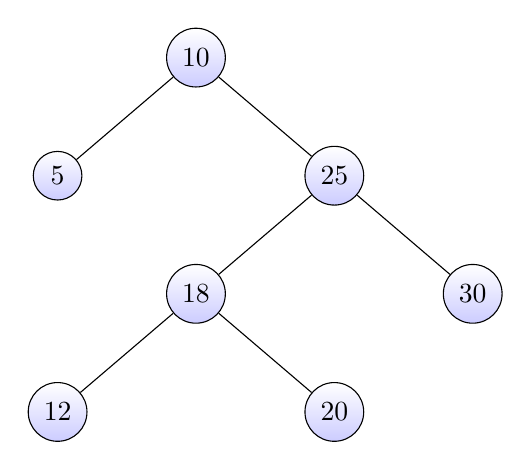
\begin{tikzpicture}[sibling distance=10em,
every node/.style = {shape=circle,
	draw, align=center,
	top color=white, bottom color=blue!20}]]
\node {10}
child { node {5} }
child { node {25}
	child { node {18}
		child { node {12} }
		child { node {20} } }
	child { node {30} } };
\end{tikzpicture}

\subsection{Implementation}
\lstset { %
	language=C++,
	backgroundcolor=\color{black!5}, % set backgroundcolor
	basicstyle=\footnotesize,% basic font setting
	tabsize=4,
}

\color{blue}
\begin{lstlisting}

class BinaryNode {
	public:
	BinaryNode* left;
	BinaryNode* right;
	BinaryNode* parent;
	int key;
};
\end{lstlisting}
\color{black}
\section{Binary Search Tree}

As the number of children of one node is at most 2 we can keep direct links to them.

For some algorithms the navigation up in the tree is required so we can keep a link to the parent node.

\section{Tries (Prefix trees)}

A \textbf{trie} is a variant of a n-ary tree in which characters are stored at each node.  

\cite{latexcompanion}

